\documentclass[addpoints,spanish, 12pt,a4paper]{exam}
%\documentclass[answers, spanish, 12pt,a4paper]{exam}
\printanswers
\pointpoints{punto}{puntos}
\hpword{Puntos:}
\vpword{Puntos:}
\htword{Total}
\vtword{Total}
\hsword{Resultado:}
\hqword{Ejercicio:}
\vqword{Ejercicio:}

\usepackage[utf8]{inputenc}
\usepackage[spanish]{babel}
\usepackage{eurosym}
%\usepackage[spanish,es-lcroman, es-tabla, es-noshorthands]{babel}


\usepackage[margin=1in]{geometry}
\usepackage{amsmath,amssymb}
\usepackage{multicol}
\usepackage{yhmath}

\pointsinrightmargin % Para poner las puntuaciones a la derecha. Se puede cambiar. Si se comenta, sale a la izquierda.
\extrawidth{-2.4cm} %Un poquito más de margen por si ponemos textos largos.
\marginpointname{ \emph{\points}}

\usepackage{graphicx}

\graphicspath{{../../img/}} 

\newcommand{\class}{2º Bachillerato CCSS}
\newcommand{\examdate}{\today}
\newcommand{\examnum}{Final 1ªEv.}
\newcommand{\tipo}{A}


\newcommand{\timelimit}{105 minutos}

\renewcommand{\solutiontitle}{\noindent\textbf{Solución:}\enspace}


\pagestyle{head}
\firstpageheader{
\includegraphics[width=0.2\columnwidth]{header_left}}{\textbf{Departamento de Matemáticas\linebreak \class}\linebreak \examnum}{
\includegraphics[width=0.1\columnwidth]{header_right}}
\runningheader{\class}{\examnum}{Página \thepage\ of \numpages}
\runningheadrule


\usepackage{pgf,tikz,pgfplots}
\pgfplotsset{compat=1.15}
\usepackage{mathrsfs}
\usetikzlibrary{arrows}


\begin{document}

\noindent
\begin{tabular*}{\textwidth}{l @{\extracolsep{\fill}} r @{\extracolsep{6pt}} }
\textbf{Nombre:} \makebox[3.5in]{\hrulefill} & \textbf{Fecha:}\makebox[1in]{\hrulefill} \\
 & \\
\textbf{Tiempo: \timelimit} & Tipo: \tipo 
\end{tabular*}
\rule[2ex]{\textwidth}{2pt}
Esta prueba tiene \numquestions\ ejercicios. La puntuación máxima es de \numpoints. 
La nota final de la prueba será la parte proporcional de la puntuación obtenida sobre la puntuación máxima. 

\begin{center}


\addpoints
 %\gradetable[h][questions]
	\pointtable[h][questions]
\end{center}

\noindent
\rule[2ex]{\textwidth}{2pt}

\begin{questions}

\question Dado el siguiente sistema:
$$\left\{ \begin{matrix}x + y + z = -2 \\ - k x + 3 y + z = -7 \\ x + 2 y + z \left(k + 2\right) = -5 \\ \end{matrix}\right.
$$
\begin{parts}
    \part[2]  Estudiar las soluciones del sistema según los valores del parámetro $k$.
    \begin{solution}
    $|A|=\left|\begin{matrix}1 & 1 & 1\\- k & 3 & 1\\1 & 2 & k + 2\end{matrix}\right|=\left(k + 1\right) \left(k + 2\right)$
    \\ - Si $k \neq -2, -1\to |A| \neq 0 \to \exists A^{-1}$ 
    \\ Como $rg(A)=rg(A^*)=3$  --> S.C.D -- > Se puede resolver por Gauss, Matriz inversa o Cramer
    \\ - Si $k=-2\to |A| = 0 \to \nexists A^{-1}$
        \\ Como $rg(A)=rg(A^*)=2 \to$  S.C.I --> Solo se puede resolver por Gauss
        \\ - Si $k=-1\to |A| = 0 \to \nexists A^{-1}$
        \\ Como $rg(A)=2 \land rg(A^*)=3 \to$  S.I. 

    \end{solution}
    \part[2]  Resolver el sistema cuando sea compatible indeterminado.
    \begin{solution}$A^*=\left(\begin{matrix}1 & 1 & 1 & -2\\2 & 3 & 1 & -7\\1 & 2 & 0 & -5\end{matrix}\right)\sim\left(\begin{matrix}1 & 1 & 1 & -2\\0 & 1 & -1 & -3\\0 & 0 & 0 & 0\end{matrix}\right)\to x=1 - 2 \lambda, y=\lambda - 3, z=\lambda$\end{solution}
\end{parts}

\question Dadas las matrices  $A=\left(\begin{matrix}k & k & k^{2}\\1 & -1 & k\\2 k & -2 & 2\end{matrix}\right)$,  $B=\left(\begin{matrix}12\\6\\8\end{matrix}\right)$
\begin{parts}
\part[2] Hallar el rango de $A$ en función de los valores de $k$.
\begin{solution} 
- Si $k \neq -1, 0, 1\to |A| \neq 0 \to \exists A^{-1} \to rg(A)=3$
- Si no $rg(A)=2$
\end{solution}
\part[2] Para $k = 2$, hallar, si existe, la solución de la ecuación $AX = B$
\begin{solution}
- Gauss: \\
$A^*=\left(\begin{matrix}2 & 2 & 4 & 12\\1 & -1 & 2 & 6\\4 & -2 & 2 & 8\end{matrix}\right)\sim\left(\begin{matrix}2 & 2 & 4 & 12\\0 & -2 & 0 & 0\\0 & 0 & -6 & -16\end{matrix}\right)\to x=\frac{2}{3}, y=0, z=\frac{8}{3}$
- Matriz inversa: \\
$A^{-1}=\left(\begin{matrix}\frac{1}{12} & - \frac{1}{2} & \frac{1}{3}\\\frac{1}{4} & - \frac{1}{2} & 0\\\frac{1}{12} & \frac{1}{2} & - \frac{1}{6}\end{matrix}\right) \to  X=A^{-1}\cdot b =\left(\begin{matrix}\frac{1}{12} & - \frac{1}{2} & \frac{1}{3}\\\frac{1}{4} & - \frac{1}{2} & 0\\\frac{1}{12} & \frac{1}{2} & - \frac{1}{6}\end{matrix}\right)\cdot \left(\begin{matrix}12\\6\\8\end{matrix}\right) =\left(\begin{matrix}\frac{2}{3}\\0\\\frac{8}{3}\end{matrix}\right)$
- Cramer: \\
$x=\frac{\left|\begin{matrix}12 & 2 & 4\\6 & -1 & 2\\8 & -2 & 2\end{matrix}\right|}{24}=\frac{16}{24}=\frac{2}{3}$ \\
$y=\frac{\left|\begin{matrix}2 & 12 & 4\\1 & 6 & 2\\4 & 8 & 2\end{matrix}\right|}{24}=\frac{0}{24}=0$ \\
$z=\frac{\left|\begin{matrix}2 & 2 & 12\\1 & -1 & 6\\4 & -2 & 8\end{matrix}\right|}{24}=\frac{64}{24}=\frac{8}{3}$
\end{solution}
\end{parts}

\question Un almacén de legumbres al por mayor tiene sacos de dos tipos, con
capacidad para 5 kg de peso y con capacidad para 10 kg de peso. Sólo tiene 180 sacos de capacidad
10 kg. Debe poner a la venta como mucho 2000 kg de alubias en sacos de ambos tipos. Por cada
3 sacos de 10 kg puede vender como mucho 2 sacos de 5 kg, y como mínimo tiene que poner a la
venta 20 sacos de 5 kg y 60 de 10 kg. Por cada saco de 10 kg obtiene un beneficio de 5 € y por
cada saco de 5 kg obtiene un beneficio de 2 €. Determine cuántos sacos de cada tipo debe vender para obtener el máximo beneficio y calcule dicho beneficio. (Justifica todos los pasos realizados)
\begin{solution}\\
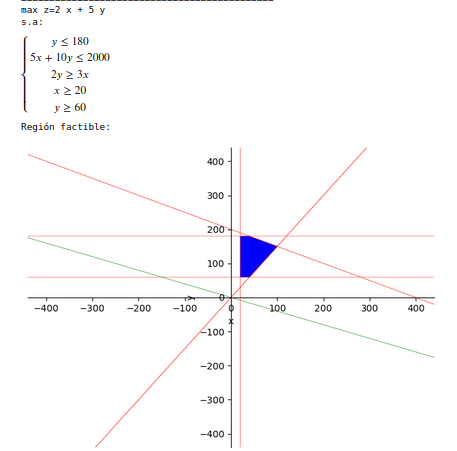
\includegraphics[scale=0.5]{prglin1}\\
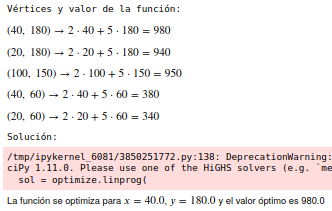
\includegraphics[scale=0.8]{prglin2}
\end{solution}

\question Una voluntaria quiere preparar helado artesano y horchata de
auténtica chufa para un rastrillo solidario. La elaboración de cada litro de helado lleva 1 hora
de trabajo y la elaboración de un litro de horchata 2 horas. Como la horchata no necesita leche,
sabe que puede preparar hasta 15 litros de helado con la leche que tiene. Para que haya suficiente
para todos los asistentes, tiene que preparar al menos 10 litros entre helado y horchata, en un
máximo de 20 horas.Si el beneficio por litro es de 25 euros para el helado y 12 euros para la horchata, obténgase
la cantidad de cada producto que se deberá preparar para maximizar el beneficio y calcúlese
el beneficio máximo que podría obtenerse (Justifica todos los pasos realizados)
\begin{solution}\\
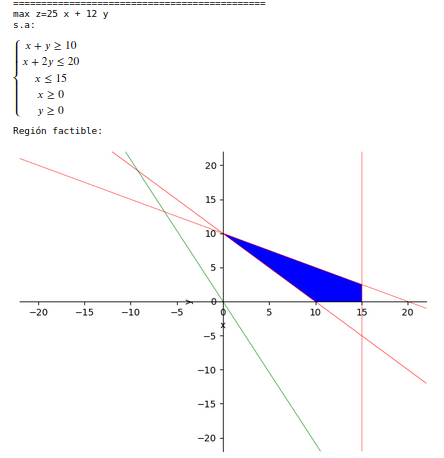
\includegraphics[scale=0.5]{prglin3}\\
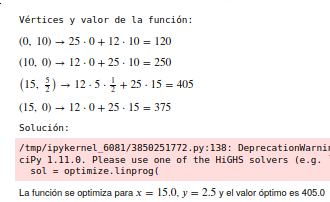
\includegraphics[scale=0.8]{prglin4}
\end{solution}

\question Dadas las matrices  $A=\left(\begin{matrix}2 & 1 & 3\\1 & -1 & 0\end{matrix}\right)$,  $B=\left(\begin{matrix}1 & -1\\2 & 0\\0 & 1\end{matrix}\right)$, $C=\left(\begin{matrix}2 & 3\\1 & 4\end{matrix}\right)$ y $D=\left(\begin{matrix}1 & 8\\0 & 5\end{matrix}\right)$ 
%\noaddpoints % to omit double points count

\begin{parts}
\part[1] Calcule $2C$ y $AB$ 

\part[2] Encontrar, si existe, una matriz $X$ tal que: $AB+2CX=D$
\begin{solution}
$AB=\left(\begin{matrix}4 & 1\\-1 & -1\end{matrix}\right)$, $2C=\left(\begin{matrix}4 & 6\\2 & 8\end{matrix}\right)$, $D-AB = \left(\begin{matrix}-3 & 7\\1 & 6\end{matrix}\right)$ y $(2C)^{-1}:\left(\begin{matrix}4 & 6\\2 & 8\end{matrix}\right)\xrightarrow{traspuesta}\left(\begin{matrix}4 & 2\\6 & 8\end{matrix}\right)\xrightarrow{adjunta}\left(\begin{matrix}8 & -6\\-2 & 4\end{matrix}\right)\xrightarrow{inversa}\left(\begin{matrix}\frac{2}{5} & - \frac{3}{10}\\- \frac{1}{10} & \frac{1}{5}\end{matrix}\right)$. \\ Por tanto, $X=(2C)^{-1}\cdot (D-AB)= \left(\begin{matrix}\frac{2}{5} & - \frac{3}{10}\\- \frac{1}{10} & \frac{1}{5}\end{matrix}\right)\cdot \left(\begin{matrix}-3 & 7\\1 & 6\end{matrix}\right)=\left(\begin{matrix}- \frac{3}{2} & 1\\\frac{1}{2} & \frac{1}{2}\end{matrix}\right)$

\end{solution}

% \part[1] Calcule, justificadamente, el rango de la matriz:$\left(\begin{matrix}1 & 0 & 2\\-1 & -1 & 1\\1 & -1 & 5\end{matrix}\right)$
% \begin{solution}
% $det(A)=0 \land $ Matriz de adjuntos $\rightarrow\left(\begin{matrix}-4 & 6 & 2\\-2 & 3 & 1\\2 & -3 & -1\end{matrix}\right)$ \\
% Por tanto, $ran(A)=2$
% \end{solution}

\end{parts}
\addpoints

% \question Resuelve el sistema: $\left(\begin{matrix}1 & 3 & -1\\1 & 2 & 0\\0 & 3 & -1\end{matrix}\right)\cdot \left(\begin{matrix}x\\y\\z\end{matrix}\right)=\left(\begin{matrix}4\\5\\3\end{matrix}\right)$

% \begin{parts}
% \part[1] Por el método de Gauss
% \part[1] Por el método de la matriz inversa
% \part[1] Por la regla de Cramer
% \end{parts}
% \begin{solution}
% $\left\{\begin{matrix}x + 3 y - z = 4\\x + 2 y = 5\\3 y - z = 3\\\end{matrix}\right.$ \\  Por Gauss: \\ $\left(\begin{matrix}1 & 3 & -1 & 4\\1 & 2 & 0 & 5\\0 & 3 & -1 & 3\end{matrix}\right)\rightarrow\left(\begin{matrix}1 & 3 & -1 & 4\\0 & -1 & 1 & 1\\0 & 0 & 2 & 6\end{matrix}\right)\to$ Sol:$\left\{\left( 1, \  2, \  3\right)\right\}$ \\ Por Matriz inversa: \\ $X=A^{-1}\cdot b=\left(\begin{matrix}1 & 0 & -1\\- \frac{1}{2} & \frac{1}{2} & \frac{1}{2}\\- \frac{3}{2} & \frac{3}{2} & \frac{1}{2}\end{matrix}\right)\cdot\left(\begin{matrix}4\\5\\3\end{matrix}\right)=\left(\begin{matrix}1\\2\\3\end{matrix}\right)$. \ Ya que $\left(\begin{matrix}1 & 3 & -1\\1 & 2 & 0\\0 & 3 & -1\end{matrix}\right)\xrightarrow{traspuesta}\left(\begin{matrix}1 & 1 & 0\\3 & 2 & 3\\-1 & 0 & -1\end{matrix}\right)\xrightarrow{adjunta}\left(\begin{matrix}-2 & 0 & 2\\1 & -1 & -1\\3 & -3 & -1\end{matrix}\right)\xrightarrow{inversa}\left(\begin{matrix}1 & 0 & -1\\- \frac{1}{2} & \frac{1}{2} & \frac{1}{2}\\- \frac{3}{2} & \frac{3}{2} & \frac{1}{2}\end{matrix}\right)$. \\ Por Cramer: \\ $det(A)=-2$ \ $\Delta_0$, $s_0$: $\left( -2, \  1\right)$ \ $\Delta_1$, $s_1$: $\left( -4, \  2\right)$ \ $\Delta_2$, $s_2$: $\left( -6, \  3\right)$ \
% \end{solution}

\question En una librería hubo la semana pasada una promoción de tres libros: una novela, un libro de
poesía y un cuento. Se vendieron 200 ejemplares de la novela, 100 de poesía y 150 cuentos. La librería ingresó por dicha promoción 8600 euros, que el precio de un ejemplar de novela es el doble que el de un cuento y que el triple de la diferencia entre el precio del ejemplar de poesía y del cuento es igual al
precio de una novela.
\begin{parts}
\part[2] Plantea un sistema de ecuaciones que refleje el enunciado

\part[1] Resuelva el problema por cualquiera de los métodos vistos en clase
\begin{solution} \\
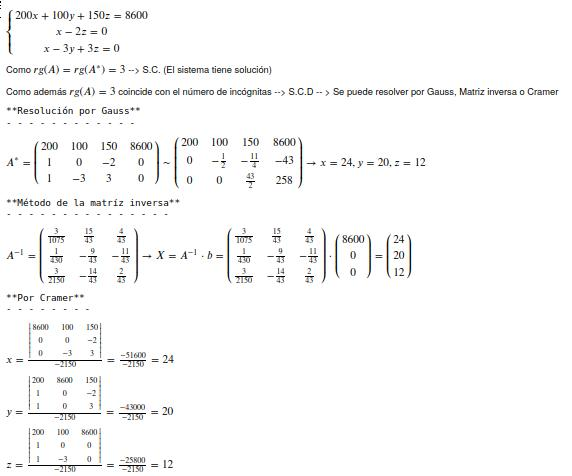
\includegraphics[scale = 0.8]{sol1}
\end{solution}
\end{parts}

% \question Un padre decide repartir su fortuna de 480 monedas de oro entre sus tres hijas: Ana,
% Carla y Pilar. La cantidad que recibe Ana
% es el doble de la suma de las cantidades que reciben Carla y Pilar. Además, la suma de
% las cantidades que reciben Ana y Pilar es igual al triple de la cantidad que recibe Carla.
% \begin{parts}
% \part[2] Plantea un sistema de ecuaciones que refleje el enunciado
% \part[1] Resuelva el problema por cualquiera de los métodos vistos en clase
% \end{parts}
% \begin{solution}
% $\left\{\begin{matrix}x + y + z = 480\\x = 2 y + 2 z\\x + z = 3 y\\\end{matrix}\right.$ \\  Por Gauss: \\ $\left(\begin{matrix}1 & 1 & 1 & 480\\1 & -2 & -2 & 0\\1 & -3 & 1 & 0\end{matrix}\right)\rightarrow\left(\begin{matrix}1 & 1 & 1 & 480\\0 & -3 & -3 & -480\\0 & 0 & 4 & 160\end{matrix}\right)\to$ Sol:$\left\{\left( 320, \  120, \  40\right)\right\}$ \\ Por Matriz inversa: \\ $X=A^{-1}\cdot b=\left(\begin{matrix}\frac{2}{3} & \frac{1}{3} & 0\\\frac{1}{4} & 0 & - \frac{1}{4}\\\frac{1}{12} & - \frac{1}{3} & \frac{1}{4}\end{matrix}\right)\cdot\left(\begin{matrix}480\\0\\0\end{matrix}\right)=\left(\begin{matrix}320\\120\\40\end{matrix}\right)$. \ Ya que $\left(\begin{matrix}1 & 1 & 1\\1 & -2 & -2\\1 & -3 & 1\end{matrix}\right)\xrightarrow{traspuesta}\left(\begin{matrix}1 & 1 & 1\\1 & -2 & -3\\1 & -2 & 1\end{matrix}\right)\xrightarrow{adjunta}\left(\begin{matrix}-8 & -4 & 0\\-3 & 0 & 3\\-1 & 4 & -3\end{matrix}\right)\xrightarrow{inversa}\left(\begin{matrix}\frac{2}{3} & \frac{1}{3} & 0\\\frac{1}{4} & 0 & - \frac{1}{4}\\\frac{1}{12} & - \frac{1}{3} & \frac{1}{4}\end{matrix}\right)$. \\ Por Cramer: \\ $det(A)=-12$ \ $\Delta_0$, $s_0$: $\left( -3840, \  320\right)$ \ $\Delta_1$, $s_1$: $\left( -1440, \  120\right)$ \ $\Delta_2$, $s_2$: $\left( -480, \  40\right)$ \ \end{solution}

\question Dado el sistema: $$\left\{\begin{matrix}x + y + z = a - 1\\a z + 2 x + y = a\\a y + x + z = 1\\\end{matrix}\right.$$
%\noaddpoints % to omit double points count
\begin{parts}
\part[2] Discutir la solución del mismo según el valor de $a$ 

% \part[1] Resolver el sistema para $a=2$

\part[3] Resolver el sistema según el valor de $a$


\end{parts}
\begin{solution}
$\left(\begin{matrix}1 & 1 & 1 & a - 1\\2 & 1 & a & a\\1 & a & 1 & 1\end{matrix}\right) \to \left(\begin{matrix}1 & 1 & 1 & a - 1\\0 & -1 & a - 2 & 2 - a\\0 & 0 & \left(a - 2\right) \left(a - 1\right) & a \left(2 - a\right)\end{matrix}\right)\to det(A)=- a^{2} + 3 a - 2\to- \left(a - 2\right) \left(a - 1\right)$. \\ \\ Discusión: \\Si a $\neq\left( 1, \  2\right)\to det(A) \neq 0 \to ran(A)=ran(A^*)=3 \to $ S.C.D. $\to$ Sol:$\left(\begin{matrix}a + 1\\\frac{2 - a}{a - 1}\\- \frac{a}{a - 1}\end{matrix}\right)$ \\Si a=1: \\ $\left(\begin{matrix}1 & 1 & 1 & 0\\0 & -1 & -1 & 1\\0 & 0 & 0 & 1\end{matrix}\right) \to ran(A^*)=3 \land ran(A)=2 \to$  S.I. \\Si a=2: \\ $\left(\begin{matrix}1 & 1 & 1 & 1\\0 & -1 & 0 & 0\\0 & 0 & 0 & 0\end{matrix}\right) \to ran(A^*)=2 \land ran(A)=2 \to$  S.C.I.  $\to$ Sol:$\left\{ x : 1 - z, \  y : 0\right\}$
\end{solution}
\addpoints



\question Dadas las siguientes restricciones: $$\left\{\begin{matrix}
2x  \leqslant  8 - y\\
x  \leqslant  3\\
y  \leqslant  4\\
x  \geqslant  0 \\
y  \geqslant  0 \\
\end{matrix}\right.$$ 
%\noaddpoints % to omit double points count

\begin{parts}
\part[1] Razonar si $z=5x+2y$ alcanza un valor máximo y uno mínimo con las restricciones anteriores. En caso afirmativo, calcular dichos valores y los puntos en los que se alcanzan.   
\begin{solution}\\
\includegraphics[scale=0.6]{fi1_1} 
\\Vértices:\\
$A(0 , 0) \to f(0,0)=0$\\
$B(3 , 0) \to f(3,0)=15$\\
$C(3 , 2) \to f(3,2)=19$\\
$D(2 , 4) \to f(2,4)=18$\\
$E(0 , 4) \to f(0,4)=8$\\
\\
Mínimo en $D$ y $f(D)=0$ \\
Máximo en $C$ y $f(C)=19$
\end{solution}
\part[1] Igual que el apartado anterior pero para $z=6x+3y$ 
\begin{solution}\\
\includegraphics[scale=0.6]{fi1_2} 
\\ Vértices:\\
$A(0 , 0) \to f(0,0)=0$\\
$B(3 , 0) \to f(3,0)=18$\\
$C(3 , 2) \to f(3,2)=24$\\
$D(2 , 4) \to f(2,4)=24$\\
$E(0 , 4) \to f(0,4)=12$\\
\\
Mínimo en $D$ y $f(D)=0$\\
Máximo en $\overline{CD}$ y $f(C)=24 \land f(D)=24$
$$\overline{CD}\equiv \left\{ \begin{matrix}
x = 3 + (2-3)\lambda \\
y = 2 + (4-2)\lambda \\
\end{matrix} , \lambda \in \left( 0, 1 \right)
\right.
$$
\end{solution}


\end{parts}

\addpoints


\question[3] Los 400 alumnos de un colegio van a ir de excursión. Para ello se contrata el viaje a una
empresa que dispone de 8 autobuses de 40 plazas y 10 con 50 plazas, pero sólo de 9 conductores para ese
día. Dada la diferente capacidad y calidad, el alquiler de cada autobús de los grandes cuesta 80 \euro. y
el de cada uno de los pequeños 60 \euro . ¿Cuántos autobuses de cada clase se tiene
que alquilar para que el coste del viaje sea mínimo?

\begin{solution}
min $z=6000 x + 8000 y$ \\
s.a: \\
$\left\{ \begin{matrix}x \leq 8  \\ y \leq 10 \\ x+y \leq 9 \\ 40x+50y \geq 400 \\ x \geq 0 \\ y \geq 0 \\ \end{matrix}\right.$ \\
Región factible:\\
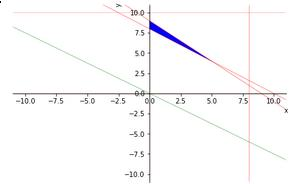
\includegraphics[scale=0.30]{region1.jpg} \\

Vértices y valor de la función: \\

(5, 4)→6000⋅5+8000⋅4=62000\\
(0, 9)→6000⋅0+8000⋅9=72000\\
(0, 8)→6000⋅0+8000⋅8=64000\\

La función se optimiza para x=5, y=4.0 y el valor óptimo es 62000
\end{solution}






% \question[3] Un camionero transporta dos tipos de mercancías, X e Y, ganando 60 y 50 euros por
% tonelada respectivamente. Al menos debe transportar 8 toneladas de X y como mucho el doble de cantidad
% que de Y. ¿A cuánto asciende su ganancia total máxima si dispone de un camión que puede transportar
% hasta 30 toneladas? 


  
% \begin{solution}
% Maximizar $f(x,y)=60x+50y$ s.a: $\left\{ \begin{matrix}
% x \geqslant 8 \\
% x \leqslant 2y \\
% x+y \leqslant 30 \\
%  \end{matrix} \right.$ 
 
% \includegraphics[scale=0.2]{sep2007}


% Vértices:\\
% $A(8 , 4) \to f(8,4)=680$\\
% $B(8 , 22) \to f(8,22)=1580$\\
% $C(20 , 10) \to f(20,10)=1700$\\

% 1700 \euro (debe transportar 20 toneladas de X y 10 toneladas de Y). \end{solution}




\addpoints



\end{questions}

\end{document}
\grid
